% !TeX root = documento.tex
% arquivo principal: compilar este (ver README.md)
\documentclass[
  12pt,
  oneside,
  a4paper,
  chapter=TITLE,
  section=TITLE,
  english,
  brazil
]{abntex2}

\usepackage[T1]{fontenc}
\usepackage[utf8]{inputenc}
\usepackage{helvet}
\renewcommand{\familydefault}{\sfdefault}
\usepackage{indentfirst}
\usepackage{graphicx}
\usepackage{float}
\usepackage{microtype}
\usepackage{booktabs}
\usepackage{tabularx}
\usepackage{xcolor}
\usepackage{pdflscape}
\usepackage{xurl}
\usepackage{tikz}
\usetikzlibrary{arrows.meta, shapes.geometric}
\usepackage[alf]{abntex2cite}

% titulos no tamanho do texto, diferenciados por negrito e caixa alta (nbr 6024)
\renewcommand{\ABNTEXchapterfont}{\bfseries}
\renewcommand{\ABNTEXchapterfontsize}{\normalsize}
\renewcommand{\ABNTEXsectionfont}{\normalfont}
\renewcommand{\ABNTEXsectionfontsize}{\normalsize}
\renewcommand{\ABNTEXsubsectionfont}{\bfseries}
\renewcommand{\ABNTEXsubsectionfontsize}{\normalsize}
\renewcommand{\ABNTEXsubsubsectionfont}{\normalfont}
\renewcommand{\ABNTEXsubsubsectionfontsize}{\normalsize}

% sumario repete o destaque de cada nivel do texto (nbr 6027)
\renewcommand{\cftsectionfont}{\normalfont}
\renewcommand{\cftsectionpagefont}{\normalfont}
\renewcommand{\cftsubsectionfont}{\bfseries}
\renewcommand{\cftsubsectionpagefont}{\bfseries}
\renewcommand{\cftsubsubsectionfont}{\normalfont}
\renewcommand{\cftsubsubsectionpagefont}{\normalfont}

\setlength{\parindent}{1.25cm}
\setlength{\parskip}{0cm}

% nome do sistema, usado no texto todo com \sistema{}
\newcommand{\sistema}{SellerHub}

\titulo{\sistema: hub de integração entre marketplaces}

\autor{
  Caio Beneton (SP3173267) \\
  Leticia Dias Rangel (SP3172384) \\
  Samuel do Prado Silva (SP3178617) \\
  Vitor Cordeiro de Souza (SP3183777)
}

% versao sem prontuario, para os metadados do pdf
\newcommand{\nomesautores}{Caio Beneton, Leticia Dias Rangel, Samuel do Prado Silva, Vitor Cordeiro de Souza}

\local{São Paulo}
\data{2026}

\instituicao{
  Instituto Federal de Educação, Ciência e Tecnologia de São Paulo \\
  Campus São Paulo \\
  Tecnologia em Análise e Desenvolvimento de Sistemas
}

\tipotrabalho{Documento técnico}

\preambulo{Documento técnico apresentado ao Instituto Federal de Educação, Ciência e Tecnologia de São Paulo, Campus São Paulo, como parte das atividades do componente curricular Projeto Integrado de Extensão, referente ao desenvolvimento e à documentação do sistema \sistema.}

\orientador{Prof. Marcelo Tavares de Santana}
%\coorientador{Prof. Nome do Coorientador}

% texto de orientacao em cinza; \mostrarorientacoesfalse tira todos do pdf
\newif\ifmostrarorientacoes
\mostrarorientacoestrue
\newcommand{\orientacao}[1]{\ifmostrarorientacoes{\color{gray}\itshape #1\par}\fi}

% dado ainda nao definido, em vermelho para nao passar despercebido
\newcommand{\pendente}[1]{\textcolor{red}{#1}}

% espaco reservado para diagrama ainda nao desenhado
% uso: \diagrama{legenda}{rotulo}, referenciado com \ref{fig:rotulo}
% quando a imagem existir em imagens/, trocar pelo ambiente figure com \includegraphics
\newcommand{\diagrama}[2]{%
  \begin{figure}[htbp]
    \centering
    \caption{#1}
    \label{fig:#2}
    \fbox{\parbox[c][5cm][c]{0.8\textwidth}{\centering\color{gray}\itshape #1 (a elaborar)}}
    \fonte{Elaborado pelos autores.}
  \end{figure}%
}

% capa: logo, instituicao e curso, autores, titulo, local e ano
\renewcommand{\imprimircapa}{%
  \begin{capa}%
    \centering
    
\includegraphics[height=3cm]{imagens/logo-ifsp.pdf}\par
    \vspace{0.5cm}
    {\bfseries\MakeUppercase{\imprimirinstituicao}\par}
    \vspace{3cm}
    {\bfseries\MakeUppercase{\imprimirautor}\par}
    \vfill
    {\bfseries\MakeUppercase{\imprimirtitulo}\par}
    \vfill
    {\bfseries\MakeUppercase{\imprimirlocal}\par}
    {\bfseries\imprimirdata\par}
    \vspace*{1cm}
  \end{capa}%
}

% folha de rosto: autores, titulo, natureza do trabalho com orientador, local e ano
\renewcommand{\folhaderostocontent}{%
  \begin{center}
    {\MakeUppercase{\imprimirautor}\par}
    \vfill
    {\bfseries\MakeUppercase{\imprimirtitulo}\par}
    \vfill
  \end{center}
  \hfill
  \begin{minipage}{.5\textwidth}
    \SingleSpacing
    \imprimirpreambulo

    \vspace{\baselineskip}
    \textbf{\imprimirorientadorRotulo}~\imprimirorientador
  \end{minipage}
  \vfill
  \begin{center}
    {\MakeUppercase{\imprimirlocal}\par}
    {\imprimirdata\par}
    \vspace*{1cm}
  \end{center}
}


% links em preto para nao destoar na impressao
\makeatletter
\hypersetup{
  pdftitle={\@title},
  pdfauthor={\nomesautores},
  pdfsubject={\imprimirtipotrabalho},
  pdfkeywords={marketplaces}{integração de sistemas}{comércio eletrônico}{gestão de anúncios},
  colorlinks=true,
  linkcolor=black,
  citecolor=black,
  filecolor=black,
  urlcolor=black,
  bookmarksdepth=4
}
\makeatother


\begin{document}
\selectlanguage{brazil}
\frenchspacing

% elementos pre-textuais
\imprimircapa
% ambiente direto: \imprimirfolhaderosto engole o comando seguinte como argumento
\begin{folhaderosto}
  \folhaderostocontent
\end{folhaderosto}
\begin{resumo}
\orientacao{Apresentar, em parágrafo único de 150 a 500 palavras, o problema do parceiro, a solução proposta, as tecnologias adotadas e os principais resultados obtidos.}

\vspace{\onelineskip}
\noindent
\textbf{Palavras-chave}: Marketplaces. Integração de sistemas. Comércio eletrônico. Gestão de anúncios.
\end{resumo}

\begin{resumo}[Abstract]
\begin{otherlanguage*}{english}
Managing sales across multiple marketplaces requires repeated product registration and the monitoring of listings, orders, and inventory in separate environments, increasing operational work and the risk of inconsistencies. This work presents the proposal and initial implementation of \sistema{}, a web application intended to centralize these activities, based on the needs of Tutymotos, a business in the motorcycle parts sector. The proposed solution includes product and listing management, order tracking, inventory control, and the analysis of business performance indicators, subject to data availability on the integrated platforms. It also includes artificial intelligence to assist with content preparation, subject to the retailer's review and approval. The procedures adopted include discussions with the administrators, observation of the store's daily operations, requirements elicitation, domain and data modeling, and the organization of the application into layers. Angular was adopted for the web interface, Go for the API, and PostgreSQL for persistence, with data access code generated by sqlc. The outcomes of this stage comprise the initial requirements, system models, and the implementation of an email and password verification flow, which does not yet include session management. All six automated interface tests, using simulated HTTP responses, passed, and static analysis of the API reported no issues. These results do not establish that the system works with the database in an integrated environment or that it provides operational gains for the store. The current contribution consists of defining the problem and building a technical foundation for the system. Assessing its effectiveness requires completing the business modules and marketplace integrations, as well as conducting tests and measurements with the retailers.

\vspace{\onelineskip}
\noindent
\textbf{Keywords}: Marketplaces. Systems integration. E-commerce. Listing management.
\end{otherlanguage*}
\end{resumo}


\pdfbookmark[0]{\listfigurename}{lof}
\listoffigures*
\cleardoublepage

\pdfbookmark[0]{\listtablename}{lot}
\listoftables*
\cleardoublepage

\begin{siglas}
  \item[API] \textit{Application Programming Interface}
  \item[HTTP] \textit{Hypertext Transfer Protocol}
  \item[IFSP] Instituto Federal de Educação, Ciência e Tecnologia de São Paulo
  \item[JSON] \textit{JavaScript Object Notation}
  \item[REST] \textit{Representational State Transfer}
  \item[SQL] \textit{Structured Query Language}
  \item[UML] \textit{Unified Modeling Language}
\end{siglas}


\pdfbookmark[0]{\contentsname}{toc}
\tableofcontents*
\cleardoublepage

% elementos textuais
\textual
% so o numero da pagina no canto superior direito, sem cabecalho
\pagestyle{simple}
\chapter{Introdução}
\label{cap:introducao}

\orientacao{Este capítulo apresenta o projeto de forma geral, estabelecendo seus objetivos, sua justificativa, seu escopo e a organização do documento. Sua função é fornecer ao leitor uma visão inicial que permita compreender o propósito e a abrangência do trabalho antes de entrar no contexto e nos aspectos técnicos.}

\section{Caracterização do Projeto}
\orientacao{Apresentar uma descrição geral do projeto, caracterizando sua natureza, finalidade, origem e principais características, de modo a situar o leitor antes da apresentação dos objetivos, da justificativa e do escopo.}

\section{Objetivos}
\orientacao{Apresentar os objetivos que orientam o desenvolvimento do projeto e delimitam os resultados que se pretende alcançar.}

\subsection{Objetivo Geral}
\orientacao{Descrever, de forma ampla, o principal resultado pretendido com o desenvolvimento do projeto.}

\subsection{Objetivos Específicos}
\orientacao{Relacionar os resultados parciais ou etapas necessárias para alcançar o objetivo geral.}

\section{Justificativa}
\orientacao{Apresentar as razões que justificam a realização do projeto, considerando sua relevância para o público atendido, para a comunidade e para a formação dos estudantes.}

\section{Escopo do Projeto}
\orientacao{Delimitar o que faz parte do projeto e, quando necessário, o que está explicitamente fora de seu escopo.}

\section{Estrutura do Documento}
\orientacao{Apresentar brevemente a organização do documento do projeto, indicando o conteúdo e a finalidade de suas principais seções.}

\chapter{Contexto do Projeto}
\label{cap:contexto}

\orientacao{Este capítulo apresenta o contexto real no qual o projeto está inserido, caracterizando o cenário, o público envolvido, as necessidades identificadas e as regras de negócio do domínio. Sua função é estabelecer a compreensão do problema sob a perspectiva da comunidade atendida antes de apresentar a solução computacional.}

\orientacao{Incluir estudo sobre a área de atuação do parceiro do projeto, mercado, índices, demandas, etc.}

\section{Cenário}
\orientacao{Descrever o contexto em que o projeto será aplicado, incluindo as características relevantes do ambiente, organização, atividade ou situação que originou a demanda.}

\section{Público-Alvo}
\orientacao{Caracterizar as pessoas, grupos ou organizações que utilizarão, serão atendidos ou serão diretamente afetados pelo projeto.}

\section{Necessidades Identificadas}
\orientacao{Apresentar as necessidades observadas no contexto do projeto que motivaram a proposição da solução, sem ainda detalhar os requisitos do sistema.}

\section{Regras de Negócio}
\orientacao{Enunciar e discutir as regras, condições, políticas e restrições próprias do domínio que devem ser respeitadas pela solução, mantendo a descrição em nível conceitual e independente da implementação.}

\begin{landscape}
\begin{figure}[htbp]
    \centering
    \caption{Diagrama de atividades do cadastro e da publicação de anúncio}
    \label{fig:atividades}
    \resizebox{\linewidth}{!}{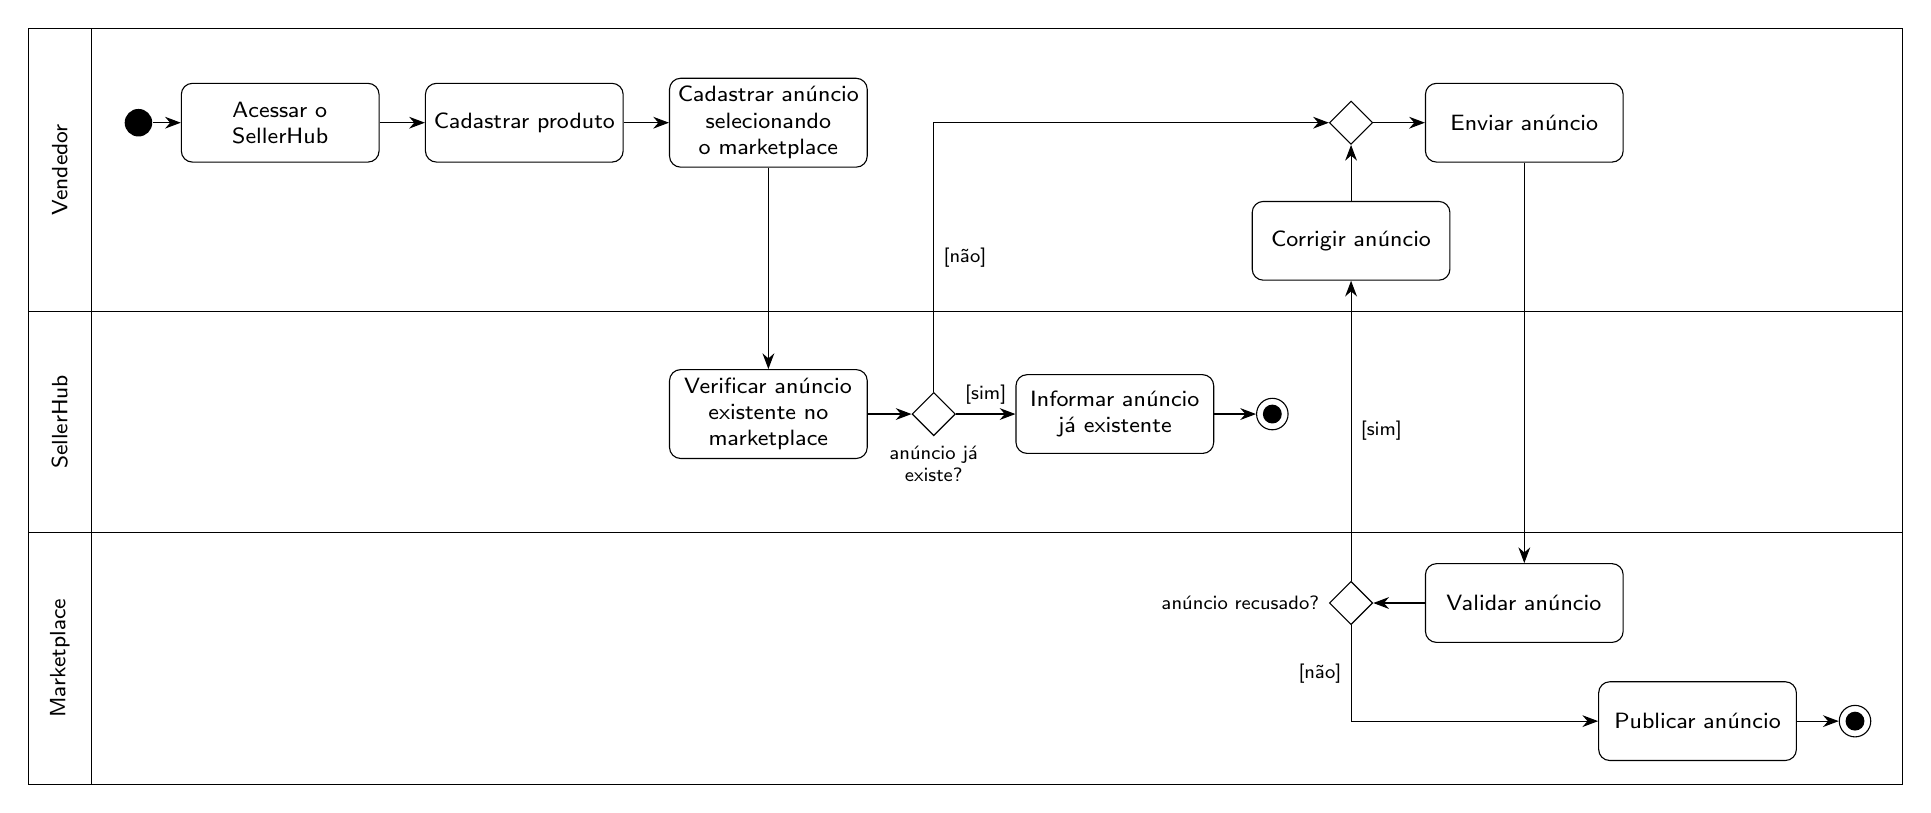
\begin{tikzpicture}[
  font=\footnotesize,
  acao/.style={draw, rounded corners=4pt, text width=2.3cm, align=center, minimum height=1cm, inner sep=3pt,
    execute at begin node={\hyphenpenalty=10000}},
  ponto/.style={draw, diamond, minimum size=0.55cm, inner sep=0pt},
  inicio/.style={circle, fill=black, minimum size=0.35cm, inner sep=0pt},
  final/.style={circle, draw, minimum size=0.4cm, inner sep=0pt},
  fluxo/.style={-{Stealth[length=2mm]}},
  guarda/.style={font=\scriptsize},
]
  % raias
  \draw (0,0) rectangle (23.8,9.6);
  \draw (0,6.0) -- (23.8,6.0);
  \draw (0,3.2) -- (23.8,3.2);
  \draw (0.8,0) -- (0.8,9.6);
  \node[rotate=90] at (0.4,7.8) {Vendedor};
  \node[rotate=90] at (0.4,4.6) {\sistema};
  \node[rotate=90] at (0.4,1.6) {Marketplace};

  % cadastro
  \node[inicio] (ini) at (1.4,8.4) {};
  \node[acao] (acessar) at (3.2,8.4) {Acessar o \sistema};
  \node[acao] (produto) at (6.3,8.4) {Cadastrar produto};
  \node[acao] (anuncio) at (9.4,8.4) {Cadastrar anúncio selecionando o marketplace};

  % verificacao de anuncio existente
  \node[acao] (verificar) at (9.4,4.7) {Verificar anúncio existente no marketplace};
  \node[ponto] (d0) at (11.5,4.7) {};
  \node[guarda, anchor=north, align=center] at (d0.south) {anúncio já\\existe?};
  \node[acao] (informar) at (13.8,4.7) {Informar anúncio já existente};
  \node[final] (fim1) at (15.8,4.7) {};
  \fill (fim1.center) circle (0.12cm);

  % envio, validacao e publicacao
  \node[ponto] (m1) at (16.8,8.4) {};
  \node[acao] (enviar) at (19.0,8.4) {Enviar anúncio};
  \node[acao] (corrigir) at (16.8,6.9) {Corrigir anúncio};
  \node[acao] (validar) at (19.0,2.3) {Validar anúncio};
  \node[ponto] (d1) at (16.8,2.3) {};
  \node[guarda, anchor=east] at (d1.west) {anúncio recusado?};
  \node[acao] (publicar) at (21.2,0.8) {Publicar anúncio};
  \node[final] (fim2) at (23.2,0.8) {};
  \fill (fim2.center) circle (0.12cm);

  \draw[fluxo] (ini) -- (acessar);
  \draw[fluxo] (acessar) -- (produto);
  \draw[fluxo] (produto) -- (anuncio);
  \draw[fluxo] (anuncio) -- (verificar);
  \draw[fluxo] (verificar) -- (d0);
  \draw[fluxo] (d0) -- node[guarda, above] {[sim]} (informar);
  \draw[fluxo] (informar) -- (fim1);
  \draw[fluxo] (d0) |- node[guarda, pos=0.25, right] {[não]} (m1);
  \draw[fluxo] (m1) -- (enviar);
  \draw[fluxo] (enviar) -- (validar);
  \draw[fluxo] (validar) -- (d1);
  \draw[fluxo] (d1) -- node[guarda, right] {[sim]} (corrigir);
  \draw[fluxo] (corrigir) -- (m1);
  \draw[fluxo] (d1) |- node[guarda, pos=0.25, left] {[não]} (publicar);
  \draw[fluxo] (publicar) -- (fim2);
\end{tikzpicture}
}
    \fonte{Elaborado pelos autores.}
\end{figure}
\end{landscape}

\chapter{Análise do Sistema}
\label{cap:analise}

\orientacao{Este capítulo transforma a compreensão do contexto e das necessidades em uma visão estruturada do sistema a ser desenvolvido. Sua função é definir o que o sistema deve fazer, quem interage com ele, quais conceitos compõem seu domínio e quais requisitos e restrições devem ser considerados, sem ainda detalhar sua implementação.}

\section{Visão Geral do Sistema}
\orientacao{Apresentar uma visão macroscópica da solução proposta, delimitando o sistema e sua finalidade antes do detalhamento de suas funcionalidades e estruturas.}

\section{Atores Envolvidos}
\orientacao{Identificar os atores que interagem diretamente com o sistema e caracterizar seus respectivos papéis.}

\section{Casos de Uso}
\orientacao{Identificar e descrever as funcionalidades do sistema sob a perspectiva dos atores, incluindo os comportamentos esperados e os fluxos relevantes.}

\diagrama{Diagrama de casos de uso}{casos-de-uso}

\section{Modelo Conceitual}
\orientacao{Representar os principais conceitos do domínio, suas características e relacionamentos, sem incorporar decisões específicas de implementação.}

\diagrama{Diagrama de classes conceitual}{classes-conceitual}

\section{Requisitos Funcionais}
\orientacao{Especificar de forma objetiva os serviços e comportamentos que o sistema deverá oferecer para atender às necessidades identificadas.}

\section{Requisitos Não Funcionais}
\orientacao{Especificar as características, qualidades e restrições que o sistema deverá atender, além das funcionalidades propriamente ditas.}

\section{Restrições do Sistema}
\orientacao{Registrar limitações impostas ao desenvolvimento ou à operação do sistema, sejam elas técnicas, institucionais, legais, orçamentárias ou decorrentes do contexto do projeto.}

\chapter{Projeto do Sistema}
\label{cap:projeto}

\orientacao{Este capítulo define como a solução será estruturada para atender aos requisitos identificados na análise. Sua função é transformar o modelo conceitual em uma especificação técnica da solução, estabelecendo sua arquitetura, componentes, dados, interfaces, interações, tecnologias e mecanismos de segurança.}

\section{Arquitetura do Sistema}
\orientacao{Apresentar a organização geral da solução, definindo seus principais elementos, responsabilidades e relações em nível arquitetural.}

\diagrama{Diagrama de componentes}{componentes}

\section{Projeto dos Componentes}
\orientacao{Detalhar a estrutura e as responsabilidades dos principais componentes definidos na arquitetura, incluindo suas interfaces e relações.}

\section{Modelo de Dados}
\orientacao{Descrever a estrutura dos dados necessários ao funcionamento do sistema e suas relações, considerando as decisões de projeto adotadas.}

\diagrama{Diagrama de classes de projeto}{classes-projeto}

\section{Projeto da Interface do Usuário}
\orientacao{Apresentar a organização e o comportamento das interfaces pelas quais os usuários interagem com o sistema, incluindo protótipos ou representações visuais quando pertinentes.}

\section{Diagramas de Interação}
\orientacao{Detalhar como os elementos do sistema colaboram para realizar os comportamentos definidos, evidenciando a sequência de mensagens e responsabilidades.}

\diagrama{Diagrama de sequência}{sequencia}

\section{Tecnologias Utilizadas}
\orientacao{Relacionar as principais linguagens, frameworks, bibliotecas, sistemas gerenciadores, ferramentas e demais tecnologias adotadas, indicando sua função no projeto.}

A \autoref{tab:tecnologias} resume as tecnologias adotadas em cada camada do \sistema{} \cite{go,sqlc,postgresql,angular}.

\begin{table}[htbp]
  \centering
  \caption{Tecnologias adotadas no \sistema}
  \label{tab:tecnologias}
  \begin{tabularx}{\textwidth}{llX}
    \toprule
    \textbf{Camada} & \textbf{Tecnologia} & \textbf{Função no projeto} \\
    \midrule
    Back-end       & Go 1.27        & API REST e regras de negócio \\
    Acesso a dados & sqlc           & Geração de código Go tipado a partir de consultas SQL \\
    Banco de dados & PostgreSQL 17  & Persistência dos dados \\
    Front-end      & Angular 22     & Interface web \\
    Ambiente       & Docker Compose & Execução opcional do PostgreSQL em contêiner \\
    \bottomrule
  \end{tabularx}
  \fonte{Elaborado pelos autores.}
\end{table}

\section{Segurança e Controle de Acesso}
\orientacao{Descrever as decisões relacionadas à autenticação, autorização, controle de acesso, proteção de dados e demais mecanismos de segurança aplicáveis ao sistema.}

\diagrama{Diagrama de estados}{estados}

\chapter{Implementação}
\label{cap:implementacao}

\orientacao{Este capítulo apresenta a materialização da solução projetada em software, descrevendo o ambiente utilizado, a organização da aplicação, a implementação dos componentes, sua integração e os procedimentos de teste. Sua função é demonstrar como o projeto definido nos capítulos anteriores foi efetivamente transformado em uma solução executável e quais resultados foram obtidos.}

\section{Ambiente de Desenvolvimento}
\orientacao{Descrever o ambiente utilizado para desenvolver e executar o sistema, incluindo hardware, sistema operacional, ferramentas e configurações relevantes.}

\section{Estrutura da Aplicação}
\orientacao{Apresentar a organização dos arquivos, módulos, pacotes e demais elementos que compõem a aplicação implementada.}

\diagrama{Diagrama de pacotes}{pacotes}

\section{Implementação dos Componentes}
\orientacao{Descrever como os componentes definidos no projeto foram efetivamente implementados, destacando aspectos técnicos relevantes.}

\section{Integração dos Módulos}
\orientacao{Descrever como os diferentes módulos e componentes da aplicação foram integrados e como ocorre sua comunicação em ambiente de execução.}

\diagrama{Diagrama de implantação}{implantacao}

\section{Testes Realizados}
\orientacao{Apresentar os procedimentos de teste realizados, os aspectos avaliados e os principais resultados obtidos.}

\section{Resultados Obtidos}
\orientacao{Apresentar os resultados alcançados com a implementação e verificar em que medida eles atendem aos objetivos e às necessidades identificadas.}

\section{Limitações da Implementação}
\orientacao{Registrar limitações, funcionalidades não implementadas, problemas conhecidos e aspectos que possam exigir complementação ou evolução futura.}

\chapter{Conclusão}
\label{cap:conclusao}

\orientacao{Este capítulo encerra o documento avaliando o projeto como um todo e relacionando os resultados alcançados aos objetivos inicialmente estabelecidos. Sua função é sintetizar as principais conclusões, registrar as dificuldades encontradas e indicar possibilidades de continuidade ou evolução do trabalho.}

\section{Considerações Finais}
\orientacao{Retomar os principais aspectos do projeto e avaliar seus resultados em relação aos objetivos estabelecidos.}

\section{Dificuldades Encontradas}
\orientacao{Relatar as principais dificuldades enfrentadas durante o desenvolvimento e, quando pertinente, as soluções adotadas.}

\section{Trabalhos Futuros}
\orientacao{Indicar possíveis evoluções, melhorias, ampliações ou funcionalidades que poderão ser desenvolvidas posteriormente.}


% elementos pos-textuais
\postextual
% so entram nas referencias as entradas citadas no texto com \cite
\bibliography{referencias}

% materiais produzidos pelos autores; descomentar quando houver o primeiro
%\begin{apendicesenv}
%\partapendices
%
%\chapter{Título do apêndice}
%Conteúdo do apêndice.
%
%\end{apendicesenv}

% materiais externos, nao produzidos pelos autores; descomentar quando houver o primeiro
%\begin{anexosenv}
%\partanexos
%
%\chapter{Título do anexo}
%Conteúdo do anexo.
%
%\end{anexosenv}


\end{document}
